\begin{figure}[h!]
\centering
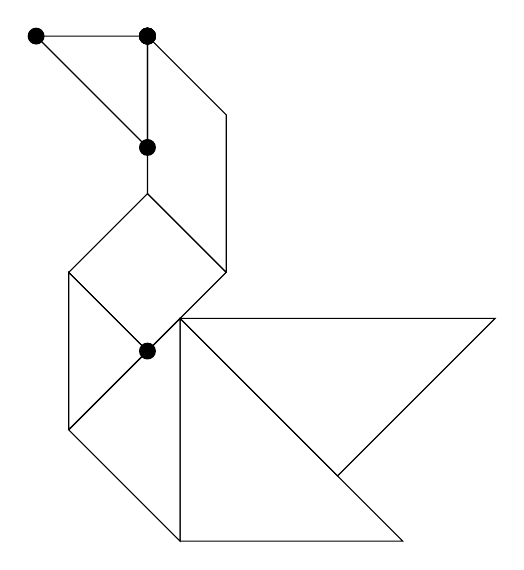
\begin{tikzpicture} %[scale=0.9]
\draw (2,0)--(4.82842,0)--(2,2.82842)--(2,0);
\draw (2,2.82842)--(6,2.82842)--(4,0.82842)--(2,2.82842);
\draw (2.585786,3.41421)--(2.585786,5.41421)--(1.585786,6.41421)--(1.585786,4.41421)--(2.585786,3.41421);
\draw (2,2.82842) -- (2,0) -- (0.585786,1.41421) -- (2,2.82842);
\draw (0.585786,1.41421)--(0.585786,3.41421)--(1.585786,2.41421)--(0.585786,1.41421);
\draw (1.585786,2.41421) -- (0.585786,3.41421) -- (1.585786,4.41421) -- (2.585786,3.41421) -- (1.585786,2.41421);
\draw (1.585786,6.41421) -- (0.171572,6.41421) -- (1.585786,5) -- (1.585786,6.41421);
\draw [fill=black](1.585786,6.41421) circle (0.1);
\draw [fill=black](1.585786,5) circle (0.1);
\draw [fill=black](0.171572,6.41421) circle (0.1);
\draw [fill=black](1.585786,2.41421) circle (0.1);
\draw [fill=black](1.585786,6.41421) circle (0.1);
\draw [fill=black](1.585786,6.41421) circle (0.1);
\draw [fill=black](1.585786,6.41421) circle (0.1);
\draw [fill=black](1.585786,6.41421) circle (0.1);
\draw [fill=black](1.585786,6.41421) circle (0.1);

\end{tikzpicture}
\caption{Segments derived when splitting at touching points from other tans}
\end{figure}